\documentclass[manuscript,screen,review]{jair}

\setcopyright{cc}
\acmDOI{10.1613/jair.1.xxxxx}
\JAIRAE{TBD}
\JAIRTrack{}
\acmVolume{TBD}
\acmArticle{TBD}
\acmMonth{TBD}
\acmYear{2026}

\RequirePackage[
  datamodel=acmdatamodel,
  style=acmauthoryear,
  backend=biber,
  giveninits=true,
  uniquename=init
]{biblatex}

\renewcommand*{\bibopenbracket}{(}
\renewcommand*{\bibclosebracket}{)}

\usepackage[T1]{fontenc}
\usepackage[utf8]{inputenc}
\usepackage{booktabs}
\usepackage{tabularx}
\usepackage{array}
\usepackage{enumitem}
\usepackage{amsmath}
\usepackage{csquotes}
\usepackage{multirow}
\usepackage{tikz}
\usetikzlibrary{arrows.meta,positioning,fit,backgrounds}

\addbibresource{lhas_refs.bib}

\begin{document}

\title[LHAS]{LHAS: A Modular and Auditable Architecture for Autonomous Literature Monitoring}

\author{Jayshree Ghorpade-Aher}
\email{jayshree.aher@mitwpu.edu.in}
\affiliation{%
  \institution{MIT World Peace University}
  \city{Pune}
  \country{India}
}

\author{Aditya Nimbalkar}
\email{1032220299@mitwpu.edu.in}
\affiliation{%
  \institution{MIT World Peace University}
  \city{Pune}
  \country{India}
}

\author{Aryan Lokare}
\email{1032222242@mitwpu.edu.in}
\affiliation{%
  \institution{MIT World Peace University}
  \city{Pune}
  \country{India}
}

\author{Chinmay Jadhav}
\email{1032221302@mitwpu.edu.in}
\affiliation{%
  \institution{MIT World Peace University}
  \city{Pune}
  \country{India}
}

\author{Shashank Kendre}
\email{1032222138@mitwpu.edu.in}
\affiliation{%
  \institution{MIT World Peace University}
  \city{Pune}
  \country{India}
}

\renewcommand{\shortauthors}{Ghorpade-Aher et al.}

\begin{abstract}
{\bf Background:}
Systematic reviews and evidence syntheses are essential for keeping pace with scientific literatures, but manual review cycles are slow, difficult to maintain, and poorly matched to fast-moving evidence streams. Existing automation tools address isolated subtasks such as screening, extraction, or summarization, yet they rarely provide a persistent, auditable state that can track how conclusions evolve over time.

{\bf Objectives:}
We introduce the Literature-based Hypothesis and Analysis System (LHAS), an autonomous literature monitoring architecture designed to ingest new papers, extract structured claims, maintain a persistent evidence graph, revise mission-level beliefs conservatively, surface contradictions explicitly, generate versioned syntheses, and monitor whether the resulting mission trajectory remains trustworthy.

{\bf Methods:}
LHAS is organized as an eight-module pipeline: query understanding, paper ingestion, claim extraction, memory, belief revision, contradiction handling, synthesis generation, and alignment monitoring. A central design choice is selective allocation of large language models (LLMs): LLMs are used only where semantic judgment is hard to replace with rules, while storage, scoring, conflict severity, confidence updates, synthesis triggering, and health monitoring are deterministic. We describe the system design, the cross-module contracts that make it auditable, and a deployment audit on a live semaglutide mission using telemetry exported from the running stack.

{\bf Results:}
On the audited mission, LHAS ingested 91 papers, produced 74 raw claims and 72 curated findings, assembled a 74-node and 202-edge claim graph, grouped 59 confirmed contradiction pairs into 2 contradiction topics, generated 2 versioned syntheses, and maintained a belief state with confidence 0.71 and dominant direction mixed. Recent hardening reduced contradiction over-penalization by shifting downstream reasoning from raw pairs to contradiction topics, and improved auditability by exposing claim- and paper-level metadata completeness summaries. The monitoring layer surfaced a BELIEF\_INERTIA alert while suppressing metadata-poor metrics rather than presenting misleading zero-valued readings.

{\bf Conclusions:}
LHAS demonstrates that autonomous literature monitoring can be organized as a stateful, auditable systems problem rather than a sequence of isolated prompts. The main practical lesson is that selective LLM usage, explicit contradiction modeling, multi-level evidence representations, and persistent mission state substantially improve traceability and operational safety. Remaining challenges include broader benchmark evaluation, tighter claim canonicalization, and richer freshness metadata for monitoring.
\end{abstract}

\begin{center}
\textbf{JAIR Reference Format:}\\
Jayshree Ghorpade-Aher, Aditya Nimbalkar, Aryan Lokare, Chinmay Jadhav, and Shashank Kendre. 2026. LHAS: A Modular and Auditable Architecture for Autonomous Literature Monitoring. \textit{Journal of Artificial Intelligence Research} TBD:TBD, TBD--TBD.
\end{center}

\received{13 April 2026}
\received[accepted]{TBD}

\maketitle

\section{Introduction}
Scientific literatures increasingly evolve on timelines that are mismatched to traditional review practice. In biomedicine and adjacent evidence-heavy domains, the number of published articles is already large enough that maintaining an up-to-date review can require substantial screening and curation effort even before synthesis begins \citep{Bastian2010}. Living systematic reviews were proposed to address this problem by shifting reviews from one-time products to continuously updated evidence assets \citep{Elliott2017}. In practice, however, living review workflows remain expensive because many of the key operations---query formulation, paper retrieval, extraction, contradiction analysis, belief updating, and synthesis rewriting---still require repeated analyst intervention.

Automation has made genuine progress on parts of this workflow. Screening systems such as Abstrackr, Rayyan, and ASReview reduce the effort of title and abstract triage \citep{Wallace2012,Ouzzani2016,vanDeSchoot2021}. Systems such as RobotReviewer and Trialstreamer automate structured extraction from clinical reports \citep{Marshall2016,Marshall2020}. A growing body of NLP benchmarks addresses evidence inference, scientific fact verification, and claim retrieval \citep{Nye2018,DeYoung2020,Wadden2020}. Yet these tools are typically optimized for one stage of the pipeline. They do not maintain a durable mission state that can answer a more operational question: what does the system currently believe about a research question, why does it believe that, and how did that belief change after new evidence arrived?

LHAS addresses this gap by treating autonomous literature monitoring as a stateful systems problem. Instead of centering the design on an end-to-end summarization model, LHAS separates the problem into eight modules with explicit boundaries: query understanding, paper ingestion, claim extraction, memory, belief revision, contradiction handling, synthesis generation, and alignment monitoring. The system persists raw records, claim relationships, and mission snapshots so that every update is auditable. It also imposes a strict usage policy on LLMs: they are reserved for tasks such as semantic extraction, relation typing, contradiction verification, and prose generation, while the rest of the pipeline---confidence updates, contradiction severity, graph persistence, synthesis triggering, and health monitoring---is rule-based.

This separation is the main systems claim of the paper. We argue that an autonomous literature monitor is trustworthy only if it can distinguish between operations that require semantic flexibility and operations that benefit from deterministic reproducibility. Belief revision, for example, should not be a free-form LLM judgment because its output affects mission-wide confidence and downstream synthesis. Likewise, the oversight layer should not itself depend on an LLM to decide whether the mission is drifting. In LHAS, those responsibilities are implemented as explicit policies over persistent state.

The contributions of this paper are fourfold. First, we present an eight-module architecture for autonomous literature monitoring that integrates retrieval, extraction, contradiction handling, synthesis, and oversight into a single persistent mission loop. Second, we articulate a selective LLM allocation policy in which deterministic logic is used wherever possible and LLMs are constrained to semantically difficult subtasks. Third, we describe a multi-level evidence representation---raw claims, curated findings, contradiction topics, and mission snapshots---that makes mission evolution inspectable over time while reducing downstream sensitivity to duplicate evidence. Fourth, we report a deployment-oriented end-to-end audit of the implemented system on a live semaglutide monitoring mission, emphasizing what the current implementation can verify operationally, what was hardened during deployment, and where the system remains limited.

\section{Related Work}
LHAS draws on several research traditions but does not fit cleanly into any one of them. The most immediate antecedents are tools for systematic review automation. Reviews of this area consistently describe the review pipeline as a collection of partially automatable subtasks, including search, deduplication, screening, extraction, and synthesis \citep{Tsafnat2014,Marshall2019}. Living systematic review frameworks highlight the need to update reviews continuously as new evidence arrives, but they do not prescribe how a monitoring system should represent evolving belief state internally \citep{Elliott2017}.

Screening and retrieval tools provide one important precursor. Abstrackr introduced predictive abstract screening for systematic reviews \citep{Wallace2012}. Rayyan demonstrated collaborative semi-automated screening in practice \citep{Ouzzani2016}, and ASReview emphasized active-learning-based prioritization of records for large evidence searches \citep{vanDeSchoot2021}. These systems are effective at narrowing the manual screening burden, but they stop short of maintaining a durable claim graph or updating mission-level conclusions over time.

Information extraction systems provide a second precursor. RobotReviewer automates risk-of-bias and study-attribute extraction from clinical trial reports \citep{Marshall2016}, while Trialstreamer operationalizes continuous extraction and indexing of clinical trial results \citep{Marshall2020}. Biomedical NLP benchmarks such as EBM-NLP and Evidence Inference focus on structured extraction of interventions, comparators, outcomes, and evidence relations \citep{Nye2018,DeYoung2020}. Scientific verification and exploratory systems such as SciFact and SciSight further show how claims and documents can be connected into evidence-centric interfaces \citep{Wadden2020,Hope2020}. LHAS builds on this line of work but differs in two ways: it uses extraction as one stage in a larger stateful loop, and it couples extraction to conservative belief revision rather than directly to a final summary.

Belief maintenance and revision form a third relevant line of work. Truth maintenance systems and belief revision frameworks have long emphasized that knowledge bases should record dependencies and support principled revision when new evidence arrives \citep{Doyle1979,AGM1985,KatsunoMendelzon1992}. LHAS adapts that intuition to literature monitoring. However, unlike classical belief revision, the underlying evidence units here are noisy, heterogeneous, and externally sourced scientific claims rather than symbolic propositions in a fully specified logic. This motivates a hybrid design in which contradictions are identified through contextual and semantic checks, but confidence updates and escalation rules remain deterministic.

Contradiction detection in scientific text is itself a growing area. Datasets and analyses of conflicting biomedical claims show that apparent contradictions often arise from population, condition, or methodological differences rather than from genuine incompatibility \citep{AlamriStevenson2016}. LHAS operationalizes this observation by requiring contextual reconciliation before confirming a contradiction. This contrasts with simpler disagreement heuristics that treat opposite direction labels as sufficient.

Finally, LHAS is related to recent LLM-based survey and synthesis systems, many of which generate fluent summaries from retrieved papers but expose limited internal state. We intentionally take a different design path. Instead of trusting an LLM to decide what the evidence means end to end, LHAS uses LLMs only for semantically difficult intermediate decisions and keeps scoring, state transitions, and monitoring deterministic. The resulting system is closer in spirit to an auditable control loop than to a one-shot review generator.

\section{System Architecture}
LHAS operates as an event-driven mission loop. A mission begins with a research question and domain context. Query understanding converts that problem statement into a structured mission representation and search plan. Paper ingestion executes search and acquisition, claim extraction turns retrieved documents into structured evidence objects, memory stores both raw and derived state, contradiction handling and belief revision update mission-level interpretation, synthesis generation produces a human-readable conclusion, and alignment monitoring evaluates whether the mission trajectory remains plausible.

Figure~\ref{fig:architecture} summarizes this architecture. The key design principle is that every module emits explicit artifacts that can be inspected independently. This reduces the risk that a failure in one stage silently contaminates the entire mission.

\begin{figure*}[t]
  \centering
  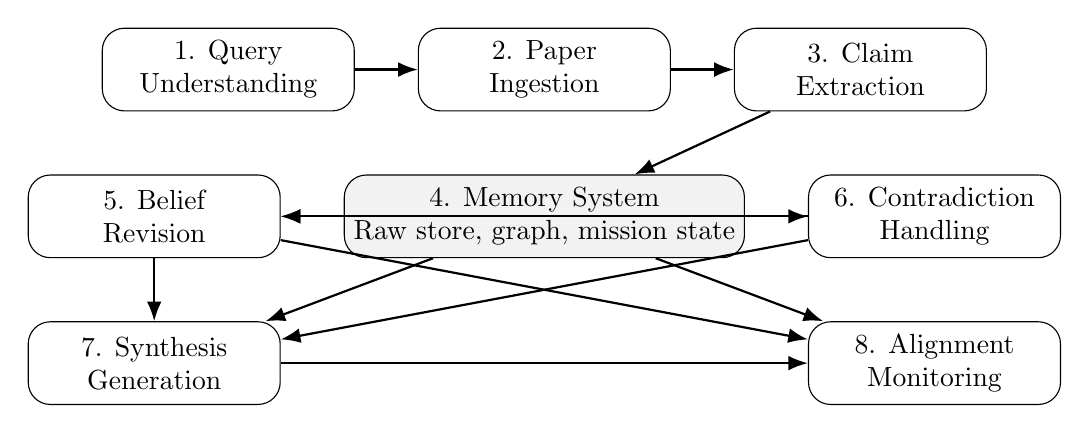
\begin{tikzpicture}[
    node distance=0.8cm and 0.8cm,
    module/.style={draw, rounded corners=8pt, fill=white, minimum width=3.2cm, minimum height=1.05cm, align=center},
    store/.style={draw, rounded corners=8pt, fill=gray!10, minimum width=4.0cm, minimum height=1.05cm, align=center},
    line/.style={-{Latex[length=2.5mm]}, thick}
  ]
    \node[module] (q) {1. Query\\Understanding};
    \node[module, right=of q] (p) {2. Paper\\Ingestion};
    \node[module, right=of p] (c) {3. Claim\\Extraction};
    \node[store, below=of p] (m) {4. Memory System\\Raw store, graph, mission state};
    \node[module, left=of m] (b) {5. Belief\\Revision};
    \node[module, right=of m] (x) {6. Contradiction\\Handling};
    \node[module, below=of b] (s) {7. Synthesis\\Generation};
    \node[module, below=of x] (a) {8. Alignment\\Monitoring};

    \draw[line] (q) -- (p);
    \draw[line] (p) -- (c);
    \draw[line] (c) -- (m);
    \draw[line] (m) -- (b);
    \draw[line] (m) -- (x);
    \draw[line] (b) -- (s);
    \draw[line] (x) -- (s);
    \draw[line] (m) -- (s);
    \draw[line] (m) -- (a);
    \draw[line] (b) -- (a);
    \draw[line] (s) -- (a);
    \draw[line] (x) -- (b);
  \end{tikzpicture}
  \caption{The LHAS pipeline. Modules communicate through explicit persistent state in the memory system rather than through ephemeral prompt context alone. Belief revision, contradiction handling, synthesis generation, and alignment monitoring all read from shared mission state but update different artifacts.}
  \Description{A left-to-right pipeline from query understanding to paper ingestion to claim extraction. Beneath those modules is a central memory system box. Belief revision and contradiction handling read from memory, synthesis generation reads from memory plus those modules, and alignment monitoring observes memory, belief revision, and synthesis generation.}
  \label{fig:architecture}
\end{figure*}

The most important architectural decision is selective LLM allocation. Table~\ref{tab:modules} shows where LLMs are used and where deterministic logic is deliberately enforced. The goal is not to minimize LLM usage for its own sake; rather, the goal is to reserve LLMs for operations that genuinely require semantic flexibility while keeping mission state transitions reproducible and inspectable.

\begin{table*}[t]
  \caption{LHAS modules, core outputs, and LLM allocation policy.}
  \label{tab:modules}
  \centering
  \begin{tabularx}{\textwidth}{@{}>{\raggedright\arraybackslash}p{2.4cm}>{\raggedright\arraybackslash}X>{\raggedright\arraybackslash}p{3.8cm}>{\raggedright\arraybackslash}p{3.6cm}@{}}
    \toprule
    Module & Main output & LLM-mediated steps & Deterministic steps \\
    \midrule
    Query understanding & Structured mission specification & Query interpretation, term expansion & Schema validation, mission typing \\
    Paper ingestion & Retrieved paper set and ingestion records & Query expansion, selective quality scoring & API orchestration, deduplication, acquisition bookkeeping \\
    Claim extraction & Structured claims with provenance & Extraction, normalization fallback, selective verification & Section scoring, confidence aggregation, validation \\
    Memory system & Raw store, graph, mission snapshots & Link type classification only & Persistence, edge weighting, contradiction indexing, checkpointing \\
    Belief revision & Updated mission belief state & Human-readable rationale only & Intake filters, decision table, confidence formulas, escalation guards \\
    Contradiction handling & Confirmed contradiction records & Ambiguous population comparison, semantic contradiction verification & Candidate retrieval, direction checks, contextual asymmetry, severity classification \\
    Synthesis generation & Versioned mission synthesis & Narrative synthesis writing & Evidence package assembly, tiering, confidence framing, validation, fallback \\
    Alignment monitoring & Monitoring snapshots and alerts & Optional benchmark disagreement analysis only & Metrics, thresholds, alert lifecycle, health classification \\
    \bottomrule
  \end{tabularx}
\end{table*}

Two additional design choices follow from this allocation policy. First, LHAS treats persistence as a first-class subsystem rather than an implementation detail. Every claim, contradiction, revision, synthesis, and monitoring snapshot is stored with enough metadata to reconstruct why the system arrived at a given conclusion. Second, LHAS explicitly distinguishes between operational state and prose. The synthesis is the only narrative artifact meant for direct human consumption; everything else is stored as structured data that can be rendered into dashboards, graphs, timelines, or audit views.

\subsection{Cross-Module Contracts}
An autonomous monitoring pipeline becomes hard to debug when adjacent modules exchange loosely specified prompt outputs. LHAS instead uses explicit cross-module contracts. Query understanding emits structured mission context rather than prose. Paper ingestion emits normalized paper records and cycle metadata. Claim extraction emits claims with typed fields and provenance references. Contradiction handling and belief revision consume claims and graph state, then emit typed records and events rather than rewriting the same objects in place. Synthesis generation consumes a deterministic evidence package, and alignment monitoring consumes persisted records rather than transient prompts.

These contracts matter for two reasons. First, they localize failure. If contradiction handling starts producing inflated pair counts, the problem can be inspected at the candidate-pair and topic-grouping layers without reverse-engineering synthesis text. Second, they enable progressively stronger interfaces. The same memory records that power the operator dashboard also support experimental evaluation, because the system stores operational truth in one place instead of scattering it across prompts and UI logic.

\subsection{Operational Loop and Recovery}
LHAS also treats mission execution as a recoverable loop rather than as a stateless batch job. At the end of a cycle, the system writes a checkpoint containing the latest mission snapshot, graph state, canonical indices, and pending events. If a later step such as synthesis generation fails, the mission can continue through a validated fallback path or resume from the last good checkpoint. This is a practical systems concern rather than a cosmetic one: literature-monitoring missions may run for days or weeks, and forcing re-extraction after every partial failure would make the system operationally fragile.

The recovery design is intentionally asymmetric. Failures in narrative generation should not corrupt stateful evidence records, and failures in monitoring should not block synthesis or ingestion. By contrast, failures in writing belief revisions or contradiction records are treated more strictly, because these are state transitions that would otherwise leave the mission inconsistent. This asymmetry reflects the relative importance of the artifacts being written.

\section{Module Descriptions}
This section describes the implemented LHAS modules in pipeline order. For each module, we focus on design choices and interfaces rather than reiterating the dashboard surface.

\subsection{Query Understanding}
The query understanding module converts a free-form mission prompt into a structured mission object containing the normalized question, domain, query type, expected evidence shape, and a search plan. In the current implementation, this module uses an LLM to parse the user question into a strict JSON schema. The schema includes fields such as the mission category, temporal hints, intervention and outcome terms, and expanded search keywords.

The design rationale is straightforward: user questions are semantically varied and often underspecified, so a flexible language model is useful for interpreting them. However, the module does not directly control retrieval. Instead, the LLM output is validated against the schema and used to generate downstream search inputs. This means that query understanding is allowed to be semantically rich but not operationally unconstrained.

The module outputs a mission record and a set of query expansions. These are consumed by paper ingestion. The module also stores enough metadata to let an operator inspect how a question was interpreted, which is important when missions appear biased or over-scoped. A small but consequential design choice is that query understanding also classifies the expected reasoning mode of the mission, for example descriptive versus comparative. That classification helps later modules decide how much weight to give null evidence, subgroup refinements, and condition-specific claims.

\subsection{Paper Ingestion}
Paper ingestion orchestrates search, retrieval, deduplication, metadata normalization, and acquisition. The implemented system retrieves candidate papers from multiple sources, including PubMed and Semantic Scholar, scores them for relevance and evidence quality, and stores ingestion records with source, year, score, and status metadata.

The most important design decision here is to separate acquisition from interpretation. Paper ingestion can use LLM assistance for query expansion and a limited quality-scoring layer, but it does not decide the mission conclusion. It merely assembles a paper set and records what was ingested. This separation matters because retrieval bias is a real failure mode in literature monitoring: a system can appear internally consistent while quietly finding only papers that support its current conclusion.

The implemented pipeline also makes ingestion the orchestration point for downstream processing. After new papers are acquired, claim extraction runs, contradiction handling evaluates the new claims against existing memory, belief revision updates mission state if justified, synthesis generation is triggered if needed, and the memory system finalizes a new mission cycle. This explicit orchestration makes the pipeline inspectable end to end rather than leaving downstream steps to implicit side effects.

Another design choice is to retain paper-level quality signals even when later modules reason primarily over claims. This preserves the distinction between document-level retrieval quality and claim-level evidence quality. A low-scoring paper can still contribute a useful claim, but the paper score remains valuable for audit, ranking, and future retrieval diagnostics.

\subsection{Claim Extraction}
Claim extraction is where retrieved papers become structured evidence objects. The current implementation extracts claims from section-aware text chunks, prioritizing full-text results and conclusion sections when available, while retaining abstract-only evidence when that is all a paper provides. Claims include intervention and outcome strings, canonicalized entity fields, direction labels, claim type, confidence, study design metadata, and provenance back to the originating paper and text span.

Several design choices are central here. First, extraction is retrieval-grounded rather than paper-summary-based. LHAS extracts claims from selected evidence chunks and stores those chunk references, which reduces the risk that the system attributes unsupported statements to a paper. Second, the module computes composite confidence from deterministic components layered on top of LLM outputs. Third, extraction is conservative about degraded cases: malformed or weakly grounded claims are retained in memory for auditability but can later be filtered out from belief revision.

LLMs are used for claim identification, structuring, and selective verification, because this is the stage where semantic interpretation is unavoidable. The surrounding logic, however, remains deterministic: chunk selection, section preferences, schema validation, confidence aggregation, and quality flags are all implemented without free-form model judgment. This allows later modules to rely on structured claims without having to reverse-engineer extraction behavior.

The extracted claim object is intentionally richer than what later dashboards display. In addition to the main statement, it includes study design type, canonical entity fields, direction label, confidence, normalization flags, validation status, mission relevance, and provenance. This richer internal object is necessary because later modules depend on different subsets of the fields. Belief revision cares about confidence and study design. Contradiction handling cares about canonical entities, population, and context. Synthesis generation cares about statement text, study type, and contradiction involvement. The claim schema therefore functions as a shared systems interface rather than merely an extraction output.

\subsection{Memory System}
The memory system is the persistent state layer of LHAS. It has three layers: an append-only raw store for paper and claim records, a typed relationship graph connecting claims, and mission state snapshots that capture what the system believed at each cycle. This separation prevents later inference modules from silently overwriting the historical record.

The raw layer stores paper metadata and claim objects verbatim. The graph layer stores claim nodes and relationship edges such as SUPPORTS, CONTRADICTS, REPLICATES, REFINES, and IS\_SUBGROUP\_OF. Edge weights are deterministic functions of study design parity, claim confidence, and recency. The mission layer stores belief snapshots, synthesis versions, drift summaries, checkpoints, and provenance logs. In the current deployment audit, this memory layer maintained 74 graph nodes, 202 graph edges, 1202 provenance events, and 3 restart checkpoints for a single mission.

This module deliberately minimizes LLM usage. The only LLM-mediated operation is relation typing for non-contradiction claim links. Persistence, contradiction indexing, edge weighting, checkpointing, and provenance logging are deterministic. That design is essential because memory is the audit substrate for every other module.

An important practical lesson from implementation is that memory should preserve both audit-level detail and user-level abstractions. Raw contradiction pairs are useful for forensic inspection, but users reason more naturally in terms of contradiction topics. LHAS now stores enough structure to support both. This dual representation is a recurring theme throughout the system: detailed records are preserved, but higher-level grouped views are derived for synthesis, monitoring, and interface design.

\subsection{Belief Revision}
Belief revision is the policy engine that updates mission-level confidence and direction. It receives the current belief state, newly extracted claims that passed intake filters, contradiction events, and drift metadata from memory. The module then applies a deterministic decision table that supports seven outcomes, including reinforcement, weakening, material update, escalation for review, reversal, and no update.

The primary design choice is conservatism. A single new paper should not reverse an established mission conclusion. Accordingly, LHAS uses explicit intake filters, weighted batch characterization, contradiction penalties, and bounded confidence updates. Confidence cannot rise by more than 0.12 or fall by more than 0.25 in a single cycle, and potential reversals require either a confirming second cycle or operator action. This makes the system behave more like a careful evidence monitor than like a reactive summarizer.

The current implementation uses an LLM only after the decision has been made, and only to write a short human-readable rationale for the audit log. The revision type, confidence update, direction change, escalation status, and drift guard are all deterministic. This is a central design claim of LHAS: prose may be generated by a model, but belief state transitions are not.

Recent hardening of the module also changed how contradictions are aggregated. Earlier versions could over-penalize missions because many raw contradiction pairs referred to the same underlying conflict topic. The current implementation therefore uses topic-aware contradiction summaries for mission-level updates while still preserving raw pairs for auditability. This is a good example of why stateful systems often need multiple representational levels for the same phenomenon.

\subsection{Contradiction Handling}
The contradiction module detects genuine conflicts without treating every disagreement as a contradiction. For each new claim, it first retrieves candidates through exact canonical entity matching and, when needed, embedding-based similarity search. Candidate pairs then pass through a deterministic direction check, contextual reconciliation over population and condition differences, and a study-design asymmetry screen. Only pairs that remain unresolved proceed to semantic verification.

The design motivation is that most apparent contradictions in scientific literature are not true contradictions. Different populations, interventions administered under different conditions, or large quality asymmetries can explain surface disagreement. LHAS therefore requires two gates before confirming a contradiction: contextual reconciliation must fail to explain the disagreement, and semantic verification must explicitly label the pair as a genuine contradiction.

In the current system, contradiction severity is deterministic and based on study design parity, confidence product, and population overlap. The deployed mission surfaced 59 confirmed contradiction pairs, but those raw pairs collapsed into only 2 contradiction topics after grouping. This distinction became operationally important during system hardening: downstream modules now reason primarily over contradiction topics rather than treating pair explosion as many independent scientific disputes.

The contradiction module also stores what did not become a contradiction. Context-resolved pairs and ambiguous pairs are written separately. This is important for auditability because an operator may ask why two superficially opposing papers were not flagged. A system that stores only confirmed contradictions cannot answer that question well.

\subsection{Synthesis Generation}
Synthesis generation converts current mission state into a concise, versioned, human-readable summary. The module is triggered periodically or when belief revision indicates a material enough change to justify rewriting the synthesis. Before any LLM call, LHAS deterministically assembles an evidence package containing tiered claim sets, contradiction summaries, subgroup qualifications, confidence tier, trigger type, and the previous synthesis version if one exists.

The key design choice is that the LLM is a writer, not a decision-maker. Evidence selection, contradiction inclusion, confidence framing, and change detection happen before prose generation. High-severity contradictions are mandatory inclusions. If the LLM output fails structural or content validation, the system retries once and then falls back to a template synthesis assembled directly from structured state.

This fallback path is not hypothetical. On the live audited mission, synthesis version~1 was produced through the template fallback after validation failure, whereas version~2 passed validation and was generated by the LLM. That behavior is intentional: a deterministic fallback is better than a blocked mission or an unsupported synthesis.

The module also performs deterministic change detection across synthesis versions. This lets the interface distinguish minor wording refreshes from genuinely important shifts in mission state. In a long-running mission, operators often care less about the absolute latest synthesis than about whether the synthesis changed materially and why.

\subsection{Alignment Monitoring}
Alignment monitoring is the oversight layer. It does not participate in evidence interpretation directly; instead, it watches whether the trajectory of the mission remains plausible. The implemented monitor evaluates six metric families: confidence trajectory integrity, synthesis drift, contradiction accumulation, evidence balance, evidence freshness, and revision pattern integrity. Alerts are threshold-based, lifecycle-managed, and stored in monitoring snapshots every five cycles.

The main design decision is that monitoring must be more reliable than the system it monitors. Consequently, metrics, alert thresholds, and health classifications are deterministic. LLM usage is reserved for an optional external benchmark comparison that is not required for core operation. The monitor is also conservative about missing information: if freshness or retrieval-balance metrics are under-informed by sparse metadata, the system marks them as insufficient rather than presenting them as authoritative zeros.

On the audited mission, the monitor initially surfaced both SUPPORT\_COLLAPSE and BELIEF\_INERTIA. After contradiction-topic hardening and metric reliability updates, only BELIEF\_INERTIA remained active and overall mission health improved from DEGRADED to WATCH. This illustrates the practical value of the monitoring layer: it can reveal whether poor mission health reflects true evidence problems or flaws in the monitor's own assumptions.

The monitoring design also plays a product role. Because alerts and health states are persisted alongside snapshots, the main mission dashboard can surface a concise answer to the question ``how is this mission going right now?'' without forcing the user to inspect individual claims. In other words, alignment monitoring is not just a backend guardrail; it is a core part of how LHAS communicates system state to operators.

\section{Experimental Evaluation}
LHAS is a systems paper contribution rather than a benchmark-centric extraction model. Our evaluation therefore focuses on end-to-end operational behavior, auditability, and consistency of module interactions. We report live deployment telemetry from the implemented stack and avoid claiming benchmark performance that has not yet been measured with gold labels.

\subsection{Evaluation Setup}
We audited one active LHAS mission asking: \emph{What are the long term effects of ozempic on our bodies?} In the current system, this was interpreted as a semaglutide monitoring mission in the medical domain. All numbers in this section were obtained from the running local deployment through its own APIs rather than from hand-constructed examples.

The hardware and software environment are modest: Windows~11 on an Intel i5-1135G7 CPU with 8~GB memory, Python~3.14.3 for the backend, React~19.2.4 and Vite~8.0.1 for the frontend, and Docker~29.2.1 for service orchestration. We emphasize this not as a performance claim, but because reproducibility for systems papers requires stating the execution context clearly.

Our evaluation philosophy is simple: report what the running system can substantiate now, and label everything else as future work. This is why the evaluation emphasizes mission telemetry, module interactions, alert behavior, and synthesis versioning rather than model-centric leaderboards. We believe this is the right level of evidence for a paper whose main claim is architectural and systems-oriented.

\begin{table*}[t]
  \caption{Live mission telemetry used in the deployment audit.}
  \label{tab:telemetry}
  \centering
  \begin{tabularx}{\textwidth}{@{}lXr@{}}
    \toprule
    Layer & Metric & Value \\
    \midrule
    Ingestion & Papers ingested & 91 \\
    Ingestion & Sources & 78 PubMed, 13 Semantic Scholar \\
    Ingestion & Paper score mean / median & 0.516 / 0.513 \\
    Extraction & Raw claims / curated findings & 74 / 72 \\
    Extraction & Claim confidence mean / median & 0.714 / 0.758 \\
    Extraction & Claims grounded in full-text results & 44 \\
    Extraction & Abstract-only claims & 20 \\
    Memory & Graph nodes / edges & 74 / 202 \\
    Memory & Provenance events / checkpoints & 1202 / 3 \\
    Contradiction handling & Confirmed pairs / topics & 59 / 2 \\
    Contradiction handling & High-severity pairs & 29 \\
    Belief revision & Current confidence / direction & 0.710 / mixed \\
    Belief revision & Revision count & 3 \\
    Synthesis & Version count & 2 \\
    Synthesis & Latest version word count & 236 \\
    Monitoring & Overall health / active alerts & WATCH / 1 \\
    \bottomrule
  \end{tabularx}
\end{table*}

\subsection{Evidence Quality and Grounding}
The first question is whether the extraction layer produces evidence that is grounded enough to support later modules. On the audited mission, 74 raw claims were stored and 72 were retained as curated findings. The mean composite claim confidence was 0.714 and the median was 0.758. Importantly, the system is no longer abstract-dominated: 44 claims were grounded in full-text results sections and 4 more in mixed abstract-plus-full-text evidence, compared with 20 abstract-only claims.

We interpret this as evidence that the section-aware retrieval and extraction hardening materially improved claim grounding. We do not report extraction precision or recall against a gold annotation set because such an evaluation has not yet been completed. Instead, we report the operational statistic that later modules depend on: most currently active claims are anchored in results-bearing text rather than in abstracts alone.

The remaining abstract-only fraction is still important. For some papers, especially those without accessible full text, abstract-only evidence may be unavoidable. LHAS therefore does not discard those claims outright. Instead, it preserves them with their provenance and lets downstream modules weight them appropriately. This is more useful than either extreme of trusting them as equivalent to full-text results or omitting them entirely and potentially losing evidence coverage.

\subsection{Contradiction Detection Behavior}
The contradiction module should detect meaningful conflicts without flooding the mission with spurious ones. On the audited mission, LHAS confirmed 59 raw contradiction pairs, but those pairs collapsed into 2 contradiction topics: one large semaglutide-weight-loss topic containing 58 pairs across 18 claims, and one semaglutide-adverse-events topic containing a single medium-severity pair.

This result illustrates both a strength and a limitation of the current implementation. The strength is that the system now distinguishes topic-level conflict from audit-level pair records, which makes the interface and downstream reasoning much more honest. The limitation is that broad claim canonicalization still allows contradiction pair counts to grow quickly inside large claim clusters. We therefore treat topic count, not pair count alone, as the more meaningful systems-level measure of contradiction burden.

We do not claim contradiction precision in the classical supervised-learning sense because no manually labeled contradiction set was constructed for this paper. Instead, our evidence is architectural and operational: confirmed contradictions must pass contextual reconciliation and semantic verification, and all confirmed pairs are stored with deterministic severity fields and an explicit verification history.

\subsection{End-to-End Cycle Integrity}
An autonomous monitor should be evaluated not only by local module outputs but also by whether a complete cycle leaves the mission in a coherent state. On the audited mission, the most recent cycle left the system with a consistent set of artifacts: belief state, synthesis version, memory snapshot, contradiction summary, and monitoring snapshot were all aligned on cycle numbering and mission identifiers. This matters because complex pipelines can easily drift into subtle state mismatches, especially when retries or fallbacks occur.

We also verified that module interactions respect the intended separation of concerns. Contradiction handling records conflicts but does not resolve them. Belief revision updates confidence and direction but does not overwrite synthesis text. Synthesis generation creates narrative output but does not rewrite graph state. Alignment monitoring emits alerts but does not modify evidence. These boundaries are easy to describe abstractly; verifying them in the live system is what makes them credible as a systems contribution.

\subsection{Belief Revision and Synthesis Fidelity}
Belief revision on the audited mission currently reports confidence 0.7101, dominant direction mixed, and latest revision type NO\_UPDATE. This is noteworthy because the mission still has substantial contradiction load. The active monitoring alert BELIEF\_INERTIA is therefore sensible: the system is seeing conflict, but current thresholds are conservative enough that many cycles still do not materially update the belief state.

Synthesis generation produced two versions. Version~1 used the template fallback after validation failure, demonstrating that the fallback path is operational rather than hypothetical. Version~2 passed validation and was produced by the LLM. The latest synthesis is 236 words long, is labeled MIXED confidence, and explicitly includes one high-severity contradiction topic corresponding to 25 underlying high-severity contradiction pairs. This behavior matches the intended synthesis policy: high-severity conflicts must be surfaced, but the synthesis should speak in terms of evidence conclusions rather than raw pair counts.

We treat synthesis fidelity here as consistency with structured state rather than as stylistic quality alone. The current version is faithful in three ways: it matches the mission confidence tier, it does not suppress the dominant contradiction topic, and it is linked back to the Tier~1 and Tier~2 claim sets that supported it. That is the right fidelity criterion for an evidence monitor. A fluent but unsupported paragraph would be less useful than a slightly stiffer synthesis that stays aligned with persistent state.

\subsection{Alignment Monitoring}
The alignment monitor provides a mission-level check on whether the overall trajectory is plausible. After the latest hardening pass, the monitor reports overall health WATCH with a single active BELIEF\_INERTIA alert. Contradiction acknowledgment rate is 0.4237, meaning that fewer than half of unresolved medium/high contradictions are currently surfaced in synthesis. This is below the ideal target and remains a meaningful operational warning.

Equally important, several previously misleading metrics are now flagged as insufficient rather than being displayed as zero-valued facts. Support ratio, retrieval balance, mean paper age, and recent ingestion rate are all currently metadata-limited on the audited mission. This is the correct behavior for an oversight layer: low-quality monitoring inputs should degrade gracefully rather than masquerading as strong evidence of failure.

From a systems perspective, this was one of the most important hardening results. Monitoring layers are often judged by how many alerts they fire, but a good oversight system should also know when it lacks enough information to judge. By attaching reliability status to selected metrics, LHAS avoids turning sparse metadata into unjustified confidence about mission health.

\section{Discussion}
The audited LHAS implementation already demonstrates a useful pattern for autonomous literature monitoring, but the deployment also exposes several design tensions that matter for future systems.

\subsection{What Worked Well}
Three design decisions appear especially important in practice. The first is persistent mission state. Because claims, contradictions, revisions, syntheses, and monitoring snapshots are all versioned and queryable, operators can inspect not only the current output but also the pathway by which the system arrived there. This is essential for trust in an autonomous monitor.

The second is selective LLM allocation. Restricting LLM use to semantically difficult operations reduced the amount of state that depends directly on unconstrained model output. In practice, this made failure modes easier to interpret. When the first synthesis generation failed validation, for example, the system fell back cleanly because evidence selection and confidence framing had already been computed outside the LLM.

The third is explicit contradiction modeling. Treating contradictions as first-class persistent objects changes the character of the system. Instead of presenting a single smoothed conclusion, LHAS can store conflict structure, expose it in synthesis, and use it for both belief revision and monitoring. This makes the system better aligned with real scientific practice, where unresolved conflict is itself meaningful.

\subsection{Current Limitations}
The most immediate limitation is claim canonicalization. The audited mission still concentrates many weight-loss findings into a single broad canonical topic, which then generates a large number of pairwise contradictions. Topic-level grouping mitigates the downstream effect of this inflation, but it does not solve the upstream representational problem. More granular finding consolidation is needed so that semantically near-duplicate claims do not behave as independent top-level evidence units.

The second limitation is evaluation scope. This paper reports a deployment audit rather than a benchmark suite with gold-standard labels for extraction, contradiction detection, and synthesis faithfulness. We intentionally avoid stronger empirical claims than the current evidence warrants. A full evaluation program would require annotated claim sets, manually judged contradiction pairs, and comparison against human-written syntheses or established review products.

The third limitation is metadata completeness. Alignment monitoring depends on publication years, study design quality, and directional histories being present and well calibrated. Where those metadata are sparse, the system now returns insufficient signals rather than misleading values, but the resulting monitor is necessarily less informative. In practice, this means that robustness at the monitoring layer still depends on continued hardening of upstream ingestion and extraction.

\subsection{Failure Modes and Open Problems}
The most important failure mode for a system like LHAS is quiet one-sidedness. Retrieval may continue to find relevant-looking papers while disproportionately missing contradictory or null evidence. This is exactly why alignment monitoring exists: the absence of runtime errors is not evidence that the mission is healthy.

Another open problem is how to calibrate conservatism in belief revision. LHAS intentionally updates slowly, but excessive inertia can become its own failure mode when contradictions accumulate faster than synthesis and belief state adapt. The current BELIEF\_INERTIA alert on the audited mission is an instance of this tension. Better contradiction-topic weighting and better evidence clustering should make the revision policy more responsive without making it volatile.

Finally, there is a broader research question about evaluating autonomous literature monitors as systems rather than as isolated models. A strong evaluation should measure not only extraction quality, but also whether a monitor stays aligned with the evidence trajectory, whether it surfaces uncertainty honestly, and whether operators can reconstruct why conclusions changed. We view this paper as a step toward that evaluation agenda rather than its endpoint.

\section{Conclusion}
LHAS reframes autonomous literature monitoring as a persistent, auditable systems problem. The central design idea is to separate semantic flexibility from state integrity: use LLMs where language understanding is genuinely needed, but keep scoring, revision, contradiction severity, persistence, and monitoring deterministic. The resulting architecture is not merely a summarizer over papers. It is a mission loop that remembers what it has seen, tracks where evidence conflicts, updates belief cautiously, and produces versioned syntheses with an explicit audit trail.

Our deployment audit shows that this approach is already operationally useful. LHAS can ingest and structure evidence, maintain a claim graph, detect contradiction topics, generate versioned syntheses, and monitor whether the mission is behaving plausibly. At the same time, the audit surfaces clear next steps: stronger finding consolidation, richer benchmark evaluation, and better metadata support for monitoring. We hope this framing encourages future work on literature-monitoring systems that are not only capable, but inspectable and trustworthy.

\begin{acks}
The LHAS implementation reported here benefited from repeated interactive debugging and hardening during development. The current draft intentionally reports only what the running system and stored telemetry support directly.
\end{acks}

\printbibliography

\appendix

\section{Additional Implementation Notes}
LHAS is implemented as a full-stack application with a FastAPI backend, a React frontend, PostgreSQL-backed persistent state, and auxiliary services for document parsing. The production code base organizes persistent data models under backend model definitions and module logic under service-layer components. The frontend exposes both an operator-facing mission dashboard and deeper inspection views for claims, contradictions, memory state, syntheses, and alignment monitoring.

The implemented stack also includes several safeguards that are easy to miss when only reading the user interface. First, cycle-producing modules write records before emitting downstream events. Second, multiple modules use fallback behavior rather than blocking the mission on a failed LLM call. Third, restart checkpoints are persisted so that missions can resume without re-extraction. These details matter because they determine whether the system behaves like a demo or like an operational monitor.

\section{Live Mission Telemetry Snapshot}
For completeness, we summarize additional telemetry from the audited mission that informed the discussion above.

\begin{itemize}[leftmargin=1.5em]
  \item Paper publication years ranged from 2015 to 2025.
  \item Claim direction counts were 44 positive, 12 negative, 3 null, and 13 unclear.
  \item Section grounding counts were 44 full-text results, 4 mixed abstract plus full text, 20 abstract only, and 4 full-text conclusions.
  \item The latest belief state was confidence 0.7101, direction mixed, revision type NO\_UPDATE, and drift trend stabilizing.
  \item The latest synthesis version was version~2, confidence tier MIXED, 236 words, and validation-passed without fallback.
  \item The active monitoring alert was BELIEF\_INERTIA, while other weak metrics were explicitly marked insufficient.
\end{itemize}

\section{Reproducibility Checklist for JAIR}

Select the answers that apply to this research, one per item.

\subsection*{All articles:}
\begin{enumerate}
    \item All claims investigated in this work are clearly stated. [yes]
    \item Clear explanations are given how the work reported substantiates the claims. [yes]
    \item Limitations or technical assumptions are stated clearly and explicitly. [yes]
    \item Conceptual outlines and/or pseudo-code descriptions of the AI methods introduced in this work are provided, and important implementation details are discussed. [yes]
    \item Motivation is provided for all design choices, including algorithms, implementation choices, parameters, data sets and experimental protocols beyond metrics. [yes]
\end{enumerate}

\subsection*{Articles containing theoretical contributions:}
Does this paper make theoretical contributions? [no]

\subsection*{Articles reporting on computational experiments:}
Does this paper include computational experiments? [yes]
\begin{enumerate}
    \item All source code required for conducting experiments is included in an online appendix or will be made publicly available upon publication of the paper. The online appendix follows best practices for source code readability and documentation as well as for long-term accessibility. [yes]
    \item The source code comes with a license that allows free usage for reproducibility purposes. [no]
    \item The source code comes with a license that allows free usage for research purposes in general. [no]
    \item Raw, unaggregated data from all experiments is included in an online appendix or will be made publicly available upon publication of the paper. The online appendix follows best practices for long-term accessibility. [partially]
    \item The unaggregated data comes with a license that allows free usage for reproducibility purposes. [partially]
    \item The unaggregated data comes with a license that allows free usage for research purposes in general. [partially]
    \item If an algorithm depends on randomness, then the method used for generating random numbers and for setting seeds is described in a way sufficient to allow replication of results. [NA]
    \item The execution environment for experiments, the computing infrastructure (hardware and software) used for running them, is described, including GPU/CPU makes and models; amount of memory (cache and RAM); make and version of operating system; names and versions of relevant software libraries and frameworks. [yes]
    \item The evaluation metrics used in experiments are clearly explained and their choice is explicitly motivated. [yes]
    \item The number of algorithm runs used to compute each result is reported. [no]
    \item Reported results have not been ``cherry-picked'' by silently ignoring unsuccessful or unsatisfactory experiments. [partially]
    \item Analysis of results goes beyond single-dimensional summaries of performance (e.g., average, median) to include measures of variation, confidence, or other distributional information. [yes]
    \item All (hyper-) parameter settings for the algorithms/methods used in experiments have been reported, along with the rationale or method for determining them. [partially]
    \item The number and range of (hyper-) parameter settings explored prior to conducting final experiments have been indicated, along with the effort spent on (hyper-) parameter optimisation. [NA]
    \item Appropriately chosen statistical hypothesis tests are used to establish statistical significance in the presence of noise effects. [NA]
\end{enumerate}

\subsection*{Articles using data sets:}
Does this work rely on one or more data sets (possibly obtained from a benchmark generator or similar software artifact)? [yes]
\begin{enumerate}
    \item All newly introduced data sets are included in an online appendix or will be made publicly available upon publication of the paper. The online appendix follows best practices for long-term accessibility with a license that allows free usage for research purposes. [NA]
    \item The newly introduced data set comes with a license that allows free usage for reproducibility purposes. [NA]
    \item The newly introduced data set comes with a license that allows free usage for research purposes in general. [NA]
    \item All data sets drawn from the literature or other public sources (potentially including authors' own previously published work) are accompanied by appropriate citations. [yes]
    \item All data sets drawn from the existing literature (potentially including authors' own previously published work) are publicly available. [yes]
    \item All new data sets and data sets that are not publicly available are described in detail, including relevant statistics, the data collection process and annotation process if relevant. [NA]
    \item All methods used for preprocessing, augmenting, batching or splitting data sets (e.g., in the context of hold-out or cross-validation) are described in detail. [partially]
\end{enumerate}

\subsection*{Explanations on any of the answers above (optional):}
This paper reports a live systems audit rather than a completed benchmark campaign. The code base is available, but the repository should be updated with an explicit open-source license and an exported evaluation artifact bundle before final submission. Items marked partially reflect this current packaging state rather than hidden methodological omissions.

\end{document}
